\section{Utilización y conservación: consumo responsable}

\subsection{El agua, un recurso imprescindible}

El agua es un recurso imprescindible para la vida, ya que ningún ser vivo puede sobrevivir sin ella. El agua es un bien escaso y su disponibilidad está relacionada con la calidad de vida. Sin embargo, no todas las personas tienen acceso a ella de la misma manera. Para hacer un uso responsable del agua, tenemos que tener en cuenta los datos siguientes:

\begin{enumerate}
    \item Unos 663 millones de personas no tienen acceso a agua potable, lo que supone un riesgo para la salud.
    \item El 97,5 \% del agua de la Tierra es agua salada, mientras que el resto, un 2,5 \%, es agua dulce.
    \item Cada 20 segundos fallece un niño o una niña menor de 5 años como consecuencia del consumo de agua no potable y malnutrición.
    \item Las familias en los países subdesarrollados emplean diariamente unas cinco horas para acceder al agua.
\end{enumerate}

\subsection{Medidas de ahorro y consumo responsable}

En los países desarrollados, el agua está presente en muchas de las actividades que se realizan diariamente en el hogar (aseo, higiene, limpieza...), en las localidades (limpieza, riego...), en la agricultura y ganadería, en la industria, en el ocio...

\vspace{3mm}
El uso, a veces, descontrolado que hace el ser humano del agua así como las condiciones climáticas, como la escasez de precipitaciones, hace que este recurso natural se agote.

\vspace{3mm}
Por ese motivo, es responsabilidad de todas las personas controlar ese consumo tomando medidas eficientes y responsables para asegurar el abastecimiento presente y futuro de agua potable. Así se contribuye a la mejora del medio ambiente y al ahorro en la factura del agua.

\subsection{Algunas medidas para el ahorro del agua}

\begin{figure}[!ht]
    \centering
    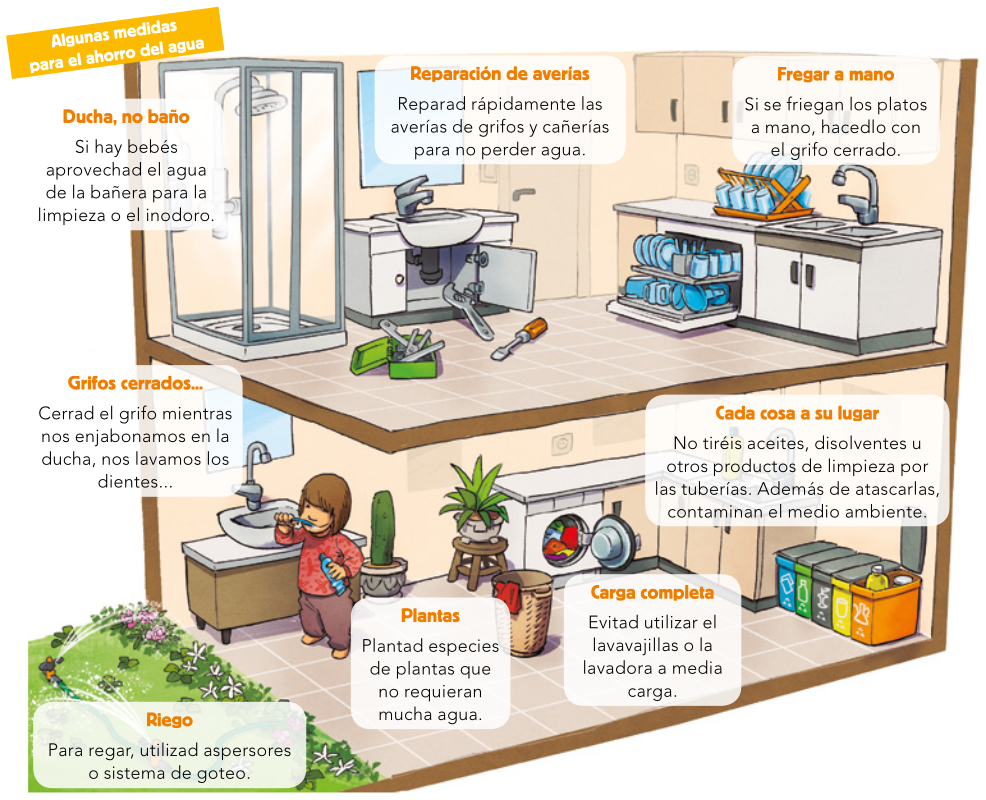
\includegraphics[width=1\linewidth]{Tema2/11_Medidas_ahorro_agua.png}
    \caption{Medidas para el ahorro del agua}
    \label{fig:medidas-ahorro-agua}
\end{figure}